% \special{dvipdfmx:config z 0}
\documentclass[UTF8,a4paper,AutoFakeBold,AutoFakeSlant]{article}
\usepackage[a4paper,left=2.8cm,right=2.6cm,top=3.7cm,bottom=3.5cm]{geometry}
\usepackage{ctex}
% \usepackage{xeCJK}
\usepackage{graphicx}
\usepackage{pythonhighlight}
\usepackage[mathscr]{eucal}
\usepackage{mathrsfs}
\usepackage{booktabs}
\usepackage{capt-of} 
\usepackage{hyperref} 
\usepackage{abstract}
\usepackage{amsmath}
\usepackage{listings}
\usepackage{color}
\usepackage{caption}
\usepackage{subfigure}
\usepackage{enumerate}
\usepackage{amsfonts} 
\usepackage{CJK,CJKnumb}
\usepackage{float}
% \usepackage{gbt7714}
\usepackage{framed}
\usepackage{multirow}
\usepackage{animate}
\usepackage[framemethod=tikz]{mdframed}



\newcommand{\song}{\CJKfamily{song}}    % 宋体   (Windows自带simsun.ttf)
\newcommand{\fs}{\CJKfamily{fs}}        % 仿宋体 (Windows自带simfs.ttf)
\newcommand{\kai}{\CJKfamily{kai}}      % 楷体   (Windows自带simkai.ttf)
\newcommand{\hei}{\CJKfamily{hei}}      % 黑体   (Windows自带simhei.ttf)
\newcommand{\li}{\CJKfamily{li}}        % 隶书   (Windows自带simli.ttf) 
\newcommand{\ssong}{\CJKfamily{STSong}}

\xeCJKsetup{SlantFactor = 0.3}
% \xeCJKsetup{SlantFactor = -0.7}
\setCJKmainfont[BoldFont=SimHei, SlantedFont=KaiTi]{SimSun}



% -- 中文字体 --
%\setCJKmainfont{Microsoft YaHei}  % 微软雅黑
%\setCJKmainfont{YouYuan}  % 幼圆
%\setCJKmainfont{NSimSun}  % 新宋体
%\setCJKmainfont{KaiTi}    % 楷体
% \setCJKmainfont{SimSun}   % 宋体
%\setCJKmainfont{SimHei}   % 黑体
% \setCJKfamilyfont{hwsong}{STSong}
 
% -- 英文字体 --
% \setmainfont{Times New Roman}
% \setmainfont{DejaVu Sans}
% \setmainfont{Latin Modern Mono}
% \setmainfont{Consolas}
% \setmainfont{Courier New}


\usepackage{xcolor}  	%高亮使用的颜色
\definecolor{commentcolor}{RGB}{85,139,78}
\definecolor{stringcolor}{RGB}{206,145,108}
\definecolor{keywordcolor}{RGB}{34,34,250}
\definecolor{backcolor}{RGB}{220,220,220}
\definecolor{shadecolor}{rgb}{0.92,0.92,0.92}   %灰色引用背景色


\usepackage{accsupp}	
\newcommand{\emptyaccsupp}[1]{\BeginAccSupp{ActualText={}}#1\EndAccSupp{}}

\usepackage{listings}
\lstset{						%高亮代码设置
	language=python, 					%Python语法高亮
	linewidth=0.95\linewidth,      		%列表list宽度
	%basicstyle=\ttfamily,				%tt无法显示空格
	commentstyle=\color{commentcolor},	%注释颜色
	keywordstyle=\color{keywordcolor},	%关键词颜色
	stringstyle=\color{stringcolor},	%字符串颜色
	%showspaces=true,					%显示空格
	numbers=left,						%行数显示在左侧
	numberstyle=\tiny\emptyaccsupp,		%行数数字格式
	numbersep=5pt,						%数字间隔
	frame=single,						%加框
	framerule=0.1pt,						%划线
	escapeinside=@@,					%逃逸标志
	emptylines=1,						%
	xleftmargin=3em,					%list左边距
	backgroundcolor=\color{backcolor},	%列表背景色
	tabsize=4,							%制表符长度为4个字符
	% gobble=4							%忽略每行代码前4个字符
}




\renewcommand{\abstractname}{}    % clear the title
\renewcommand{\absnamepos}{empty}
%去除摘要两边缩进
\makeatletter
  \renewenvironment{abstract}{%
      \if@twocolumn
        \subsection*{\abstractname}%
      \else
        \small
        \begin{center}%
          {\bfseries \abstractname\vspace{-.5em}\vspace{\z@}}%
        \end{center}%
      \fi}
      {}
  \makeatother
\lstset{
  language=Matlab,
  keywords={break,case,catch,continue,else,elseif,end,for,function,
      global,if,otherwise,persistent,return,switch,try,while},
  basicstyle=\ttfamily,
  keywordstyle=\color{blue}\bfseries,
  commentstyle=\color{dkgreen},
  stringstyle=\color{dkpurple},
  backgroundcolor=\color{white},
  tabsize=4,
  showspaces=false,
  showstringspaces=false
}

\title{\textbf{\textsf{{\textsf{LB5} \heiti{机器学习概论}}}}} 
\author{\ssong PB19151769~~~~马宇骁}
\date{}

% 去掉红框
\hypersetup{
colorlinks=true,
linkcolor=black
}

\begin{document}



\maketitle

\tableofcontents
\newpage


% ----------------------------------section----------------------------------------------


\section{实验要求}

\begin{itemize}
  \item 数据预处理:需要注意,提供数据包含大量冗余随机特征、outlier数据以及Null数据,你需要综合运用所学的知识进行数据降维、降噪、补缺、特征提取、编码以及必要的其他数据预处理工作。
  \item 数据划分:你需要将所提供的train数据集按照所学的方法拆分成训练集以及测试集。
  \item 模型训练:你需要分别使用本课程所学习的线性回归模型、决策树模型、神经网络模型、支持向量机以及XGBoost等分类模型来完成标签预测任务。
  \item 模型验证:你需要将test\_feature.csv的数据输入到一个你认为性能最佳的模型中,然后仿照train\_label.csv的文件格式生成对应标签数据文件,命名为test\_label.csv,并将它包含在你所提交的压缩包中。
  \item 实验分析:你需要仔细撰写实验报告以及相关分析。
\end{itemize}







% ----------------------------------section----------------------------------------------

\section{实验原理}

\subsection{多分类逻辑回归}

在多类别逻辑回归中,因变量是根据一系列自变量(就是我们所说的特征、观测变量)来预测得到的。具体来说,就是通过将自变量和相应参数进行线性组合之后,使用某种概率模型来计算预测因变量中得到某个结果的概率,而自变量对应的参数是通过训练数据计算得到的,有时我们将这些参数成为回归系数。

在二分类逻辑回归的基础上扩展,softmax 回归输出的 K 种类别的概率。模型公式如下:
\begin{equation*}
  h_{\theta}\left(x^{(i)}\right)=\left[\begin{array}{c}
    p\left(y^{(i)}=1 \mid x^{(i)} ; \theta\right) \\
    p\left(y^{(i)}=2 \mid x^{(i)} ; \theta\right) \\
    \vdots \\
    p\left(y^{(i)}=k \mid x^{(i)} ; \theta\right)
    \end{array}\right]=\frac{1}{\sum_{j=1}^{k} e^{\theta_{j}^{T} x^{(i)}}}\left[\begin{array}{c}
    e^{\theta_{1}^{T} x^{(i)}} \\
    e^{\theta_{2}^{T} x^{(i)}} \\
    \vdots \\
    e^{\theta_{k}^{T} x^{(i)}}
    \end{array}\right]
\end{equation*}

参数$\theta$是一个矩阵,矩阵的每一行可以看做是一个类别所对应分类器的参数,总共有 k 行,输出的 K 个数就表示该类别的概率,总和为 1。这样,softmax 回归模型对于一个测试样本,可以得到多个类别对应的概率值,模型选取概率最高的类别作为最终判定结果。



\subsection{多分类决策树}

划分数据集可以选择很多特征,那么关键问题在于现在使用哪个特征能得到最好的划分结果,因此需要对特征进行评估!
根据该特征进行数据集划分会得到很多分支,如果某个分支下的数据属于同一类型,则已经正确分类,如果不属于同一类型,继续选取此时的最好特征继续划分!
最后:所有具有相同类型的数据均在同一个数据子集内。

决策树构造过程总结为:
\begin{enumerate}
  \item 评估最好特征
  \item 划分分支
  \item 对分支继续评估最好特征+划分分支
\end{enumerate}



\subsection{神经网络}

主要使用sklearn库中的MLPClassifier直接进行模型构建。
以下是其的几个重要参数说明:
\begin{itemize}
  \item hidden\_layer\_sizes : 元组形式,长度n\_layers-2,默认(100,),第i元素表示第i个神经元的个数
  \item activation: {‘identity’, ‘logistic’, ‘tanh’, ‘relu’},默认"relu"
  \item solver:{‘lbfgs’, ‘sgd’, ‘adam’}, default ‘adam’. sgd:随机梯度下降; lbfgs:quasi-Newton方法的优化器; adam: Kingma, Diederik, and Jimmy Ba提出的机遇随机梯度的优化器
  \item alpha:float,可选的,默认0.0001,正则化项参数
  \item learning\_rate:{‘constant’,‘invscaling’, ‘adaptive’},默认‘constant’,用于权重更新,只有当solver为’sgd‘时使用
  \item max\_iter: int,可选,默认200,最大迭代次数。
  \item tol:float, 可选,默认1e-4,优化的容忍度
\end{itemize}



\subsection{支持向量机}

支持向量机(support vector machines, SVM)是一种二分类模型,它的基本模型是定义在特征空间上的间隔最大的线性分类器,间隔最大使它有别于感知机;SVM还包括核技巧,这使它成为实质上的非线性分类器。SVM的的学习策略就是间隔最大化,可形式化为一个求解凸二次规划的问题,也等价于正则化的合页损失函数的最小化问题。SVM的的学习算法就是求解凸二次规划的最优化算法。

与实验一相同(在预测的时候多分类训练和预测是利用k(k-1)/2个1v1来实现)



\subsection{XGBoost}

Boosting方法,通过将多个弱学习器集成起来形成一个强学习器。XGBoost(eXtreme Gradient Boosting)是Boosting算法中的一种,是一种提升树模型,将很多树的模型集成起来。其以正则化提升(Regularized Boosting)技术而闻名,通过代价函数里加入正则项,控制模型的复杂度,防止过拟合。可以实现并行处理,相比GBM有了很大的速度提升。







% ----------------------------------section----------------------------------------------


\section{实验实现}


\subsection{数据预处理}

由于训练数据集总共有10000条,且有120个feature,其中存在空值和异常数据,因此考虑对原始数据集进行预处理。


\subsubsection{空值填充}

按总行数来看,空值由于占比过高(45.14\%),因此不直接去除,采用上一行的值填充。
\begin{python}
  data.fillna(method='pad', axis=0)
\end{python}


\subsubsection{异常值}

通过绘制 'feature\_116' 的箱线图(图 \ref{f:异常值})发现
\begin{figure}[htbp]
	\centering
	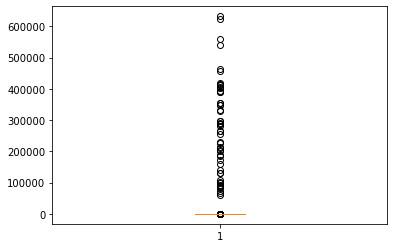
\includegraphics[scale=0.625]{异常值.png}
	\caption{116异常值}
	\label{f:异常值}
\end{figure}
异常值确实存在。因此,对于过大以及过小值做如下处理:

\begin{python}
  # 如果出现异常数据就用5%和95%的分位数取取边界值
  for obj in datanames:
      # 肉眼观察最大值都大于0
      if (max(data1[obj])>=0 and np.percentile(data1[obj], 95)>=0) and max(data1[obj]) > np.percentile(data1[obj], 95)*100:
          data1[obj][data1[obj]>np.percentile(data1[obj], 95)] = np.percentile(data1[obj], 95)
      # 最小值分类处理
      if (min(data1[obj])>=0 and np.percentile(data1[obj], 5)>=0) and np.percentile(data1[obj], 5)-min(data1[obj]) > np.percentile(data1[obj], 95)/100:
          data1[obj][data1[obj]<np.percentile(data1[obj], 5)] = np.percentile(data1[obj], 5)
      if (min(data1[obj])<0 and np.percentile(data1[obj], 5)>=0) and np.percentile(data1[obj], 5)+min(data1[obj]) < min(data1[obj])/100:
          data1[obj][data1[obj]<np.percentile(data1[obj], 5)] = np.percentile(data1[obj], 5)
      if (min(data1[obj])<0 and np.percentile(data1[obj], 5)<0) and np.abs(np.percentile(data1[obj], 5)-min(data1[obj])) > np.abs(min(data1[obj])/100):
          data1[obj][data1[obj]<np.percentile(data1[obj], 5)] = np.percentile(data1[obj], 5)
\end{python}


\subsubsection{去噪以及降维}

\begin{itemize}
  \item 小波变换去噪
\end{itemize}

将信号经小波分解后小波系数较大,噪声的小波系数较小,并且噪声的小波系数要小于信号的小波系数,通过选取一个合适的阀值,大于阀值的小波系数被认为是有信号产生的,应予以保留,小于阀值的则认为是噪声产生的,置为零从而达到去噪的目的。

选用Daubechies8小波,将信号进行小波分解,再将噪声滤波,最后将信号进行小波重构。

\begin{python}
  ## 小波变换去噪
  import pywt
  
  w = pywt.Wavelet('db8')  # 选用Daubechies8小波
  maxlev = pywt.dwt_max_level(len(data1), w.dec_len)
  threshold = 0.2  # Threshold for filtering
  for obj in datanames:
      lis = list(data1[obj])
      coeffs = pywt.wavedec(lis, 'db8', level=maxlev)  # 将信号进行小波分解
      for i in range(1, len(coeffs)):
          coeffs[i] = pywt.threshold(coeffs[i], threshold*max(coeffs[i]))  # 将噪声滤波
      datarec = pywt.waverec(coeffs, 'db8')  # 将信号进行小波重构
      data1[obj] = datarec
\end{python}

\begin{itemize}
  \item 奇异值分解降维
\end{itemize}

若要对行数据进行压缩,我们从矩阵\large A的奇异值分解式子$\large A = U\Sigma V^T$入手。
将等式两边同时乘以左奇异矩阵的转置矩阵$\large U^T$,得到$\large U^TA = U^TU\Sigma v^T = \Sigma V^T$.
左侧表达式$\large U^TA$表示把矩阵$\large A$的n个m维列向量并排放置:
\begin{equation*}
  \begin{aligned}
  \left[u_{1}, u_{2}, u_{3}, \ldots u_{m}\right]^{T} A & =\left[\begin{array}{c}
    u_{1}^{T} \\
    u_{2}^{T} \\
    u_{3}^{T} \\
    \ldots \\
    u_{m}^{T}
    \end{array}\right]\left[\operatorname{col} A_{1}, \operatorname{col} A_{2}, \text { col } A_{3}, \text { clo } A_{n}\right]\\&=\left[\begin{array}{ccccc}
    u_{1}^{T} \operatorname{col} A_{1} & u_{1}^{T} \text { col } A_{2} & u_{1}^{T} \operatorname{col} A_{3} & \ldots & u_{1}^{T} c o l A_{n} \\
    u_{2}^{T} \operatorname{col} A_{1} & u_{2}^{T} \operatorname{col} A_{2} & u_{2}^{T} \operatorname{col} A_{3} & \ldots & u_{2}^{T} c o l A_{n} \\
    u_{3}^{T} \operatorname{col} A_{1} & u_{3}^{T} \operatorname{col} A_{2} & u_{3}^{T} \operatorname{col} A_{3} & \ldots & u_{3}^{T} \operatorname{col} A_{n} \\
    \ldots & \ldots & \ldots & \ldots & \ldots \\
    u_{m}^{T} \operatorname{col} A_{1} & u_{m}^{T} \operatorname{col} A_{2} & u_{m}^{T} \operatorname{col} A_{3} & \ldots & u_{m}^{T} \operatorname{col} A_{n}
    \end{array}\right]
  \end{aligned}
\end{equation*}

此时,可以把每一列看作一个样本,各行是样本的不同特征,各行之间彼此无关,
此时可以选择最大的k个奇异值对应的k个标准正交向量,形成行压缩矩阵
$$ U_{k \times m}^{T}=\left[\begin{array}{c}
  u_{1}^{T} \\
  u_{2}^{T} \\
  u_{3}^{T} \\
  \cdots \\
  u_{k}^{T}
  \end{array}\right] $$

通过式子
$$ U_{k \times m}^{T} \operatorname{col} A_{i}=\left[\begin{array}{c}
  u_{1}^{T} \operatorname{col} A_{i} \\
  u_{2}^{T} \operatorname{col} A_{i} \\
  u_{3}^{T} \operatorname{col} A_{i} \\
  \ldots \\
  u_{k}^{T} \operatorname{col} A_{i}
  \end{array}\right] $$
实现了列向量从m维降低到k维,完成主成分提取。

\begin{figure}[htbp]
	\centering
	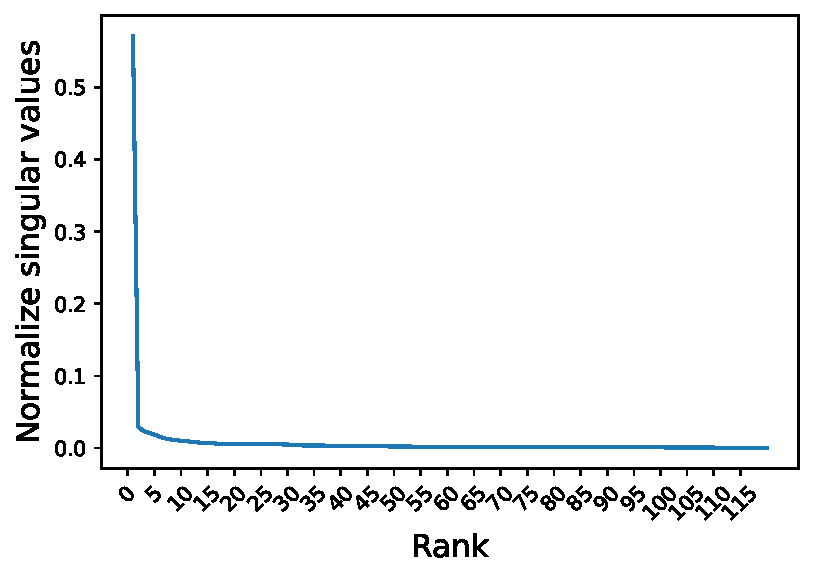
\includegraphics[scale=0.625]{svd.pdf}
	\caption{奇异值序列}
	\label{f:奇异值序列}
\end{figure}

对实验数据,经过SVD提取,其中奇异值序列归一之后如图 \ref{f:奇异值序列}.
因此,大概可以选择保留的奇异值阶数11,进行数据重构,将数据集最后转换成10000*11的维数。



\subsection{实验调试}


\subsubsection{多分类逻辑回归}

规定当相邻两次迭代的差异小于1e-3,或者超过最大迭代次数100时停止拟合,最终拟合过程如下:

\begin{mdframed}[hidealllines=true,backgroundcolor=shadecolor]
  \begin{verbatim}
    Processing:  82%|████████▏ | 82/100 [06:40<01:28,  4.94s/it]
    一共用时:488.5729990005493s
  \end{verbatim}
\end{mdframed}

预测准确率为:0.249


\subsubsection{决策树}

最大深度设置为6,
自己撰写构建决策树的拟合过程如下(此结果还是120列时候的情况(因为虽然大幅度降维之后会减少运行时间,
但不想等了)):

\begin{mdframed}[hidealllines=true,backgroundcolor=shadecolor]
  \begin{verbatim}
    Processing: 100%|██████████| 120/120 [53:52<00:00, 26.94s/it] 
    Processing: 100%|██████████| 120/120 [02:07<00:00,  1.06s/it]
    Processing: 100%|██████████| 120/120 [00:05<00:00, 23.31it/s]
    Processing: 100%|██████████| 120/120 [00:00<00:00, 489.80it/s]
    Processing: 100%|██████████| 120/120 [00:00<00:00, 1084.13it/s]
    Processing: 100%|██████████| 120/120 [00:00<00:00, 1410.85it/s]
    Processing: 100%|██████████| 120/120 [00:00<00:00, 1026.40it/s]
    Processing: 100%|██████████| 120/120 [00:00<00:00, 3115.89it/s]
    Processing: 100%|██████████| 120/120 [00:00<00:00, 2307.73it/s]
    Processing: 100%|██████████| 120/120 [00:04<00:00, 28.22it/s]
    Processing: 100%|██████████| 120/120 [00:03<00:00, 35.15it/s]
    Processing: 100%|██████████| 120/120 [00:02<00:00, 42.05it/s]
    Processing: 100%|██████████| 120/120 [00:00<00:00, 1587.78it/s]
    Processing: 100%|██████████| 120/120 [00:00<00:00, 845.01it/s]
    Processing: 100%|██████████| 120/120 [00:00<00:00, 1263.17it/s]
    Processing: 100%|██████████| 120/120 [00:00<00:00, 3000.07it/s]
    Processing: 100%|██████████| 120/120 [01:21<00:00,  1.48it/s]
    Processing: 100%|██████████| 120/120 [00:05<00:00, 21.35it/s]
    Processing: 100%|██████████| 120/120 [00:00<00:00, 810.63it/s]
    Processing: 100%|██████████| 120/120 [00:00<00:00, 827.77it/s]
    Processing: 100%|██████████| 120/120 [00:04<00:00, 25.14it/s]
    Processing: 100%|██████████| 120/120 [00:00<00:00, 294.90it/s]
    Processing: 100%|██████████| 120/120 [00:03<00:00, 37.53it/s]
    Processing: 100%|██████████| 120/120 [00:41<00:00,  2.92it/s]
    Processing: 100%|██████████| 120/120 [00:03<00:00, 31.50it/s]
    ...
    Processing: 100%|██████████| 120/120 [00:00<00:00, 3438.54it/s]
    Processing: 100%|██████████| 120/120 [00:00<00:00, 4287.67it/s]
    Processing: 100%|██████████| 120/120 [00:01<00:00, 87.72it/s]
    Processing: 100%|██████████| 120/120 [00:01<00:00, 94.32it/s] 
    Processing: 100%|██████████| 120/120 [00:00<00:00, 4283.07it/s]
    一共用时:9171.37307024002s
  \end{verbatim}
\end{mdframed}

预测准确率为:0.252


\subsubsection{神经网络}

做如下参数设置:
\begin{python}
  netmodel = MPC(verbose=False,solver='sgd', alpha=1e-5, activation='tanh',hidden_layer_sizes=(11,32,64,32,4,2), max_iter=5000, tol=1e-5, learning_rate='adaptive')
\end{python}
tanh的激活函数,6层神经网络的拟合信息如下:
一共用时:5.553001403808594s
\begin{python}
  print(netmodel.n_iter_)
  print(netmodel.loss_)
  print(netmodel.score(np.array(X_test), np.array(y_test)))
  print(netmodel.out_activation_)
\end{python}
\begin{mdframed}[hidealllines=true,backgroundcolor=shadecolor]
  \begin{verbatim}
    118
    1.3862243682913666
    0.245
    softmax
  \end{verbatim}
\end{mdframed}

预测准确率为:0.245


\subsubsection{支持向量机}

将自己写的MultiSVM参数设置为:
max\_iter = 100, epsilon=1e-5, kernel\_type='linear', C=1.0

对于此数据集,共有6个1v1的svm二分类器,对于同一条数据所有判断为一个的类进行统计,最多的作为预测值
(相同时取第一个(np.argmax的逻辑))。拟合过程如下:

\begin{mdframed}[hidealllines=true,backgroundcolor=shadecolor]
  \begin{verbatim}
    Processing: 100%|██████████| 100/100 [01:08<00:00,  1.46it/s]
    Processing: 100%|██████████| 100/100 [01:08<00:00,  1.46it/s]
    Processing: 100%|██████████| 100/100 [01:05<00:00,  1.52it/s]
    Processing: 100%|██████████| 100/100 [01:06<00:00,  1.50it/s]
    分类器::  67%|██████▋   | 4/6 [04:29<02:14, 67.13s/it]
    一共用时:403.68699979782104s
  \end{verbatim}
\end{mdframed}

预测准确率为:0.262


\subsubsection{XGBoost}

做如下参数设置:
\begin{python}
  params = {
    'booster':'gbtree',
    'objective':'multi:softmax',   # 多分类问题
    'gamma':0.1,    # 用于控制是否后剪枝的参数,越大越保守,一般0.1 0.2的样子
    'max_depth':10,  # 构建树的深度,越大越容易过拟合
    'lambda':2,  # 控制模型复杂度的权重值的L2 正则化项参数,参数越大,模型越不容易过拟合
    'subsample':0.7, # 随机采样训练样本
    'silent':0,  # 设置成1 则没有运行信息输入,最好是设置成0
    'eta':0.001,  # 如同学习率
    'seed':1000,
    'nthread':7,  #CPU线程数
    #'eval_metric':'auc'
  }
\end{python}

预测准确率为:0.255



\subsection{预测结果}

最终,综合比较下来,决定使用我的MultiSVM作为对预测集的模型。
将预测结果附在同一文件夹中。
















% \begin{figure}[H]
% 	\centering
% 	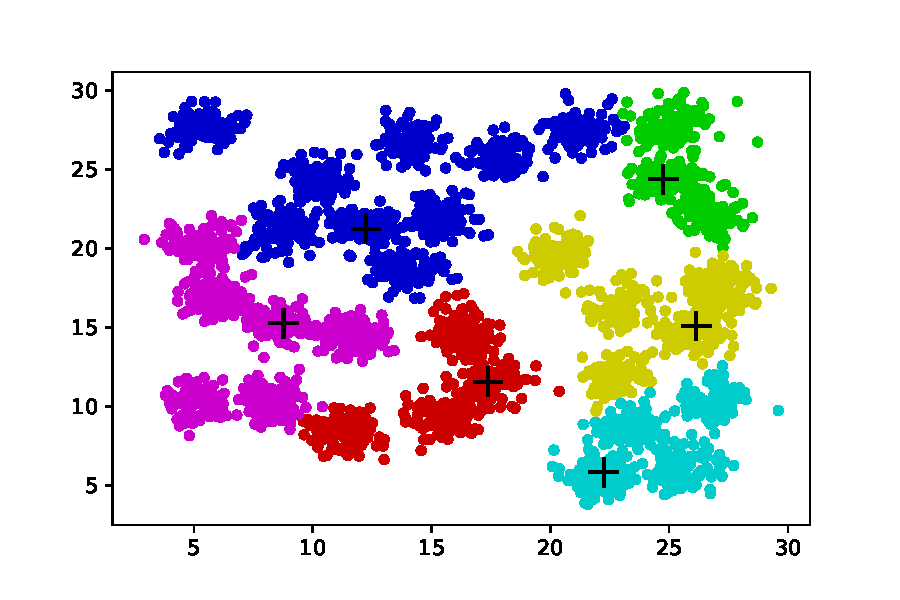
\includegraphics[scale=0.625]{cluster1.pdf}
% 	\caption{D31}
% 	\label{f:D31}
% \end{figure}





















% \bibliographystyle{gbt7714-numerical}
% % \bibliographystyle{7714-author-year}
% \bibliographystyle{ieeetr}
% \bibliography{bibl}

\end{document}